%\setbeameroption{notes on second screen} %Dual-Screen Notes
%\setbeameroption{show only notes} %Notes Output

% white on black
\setbeamercolor{normal text}{fg=white,bg=blue!20!black}
\setbeamercolor{structure}{fg=white}
\setbeamercolor{alerted text}{fg=red!85!black}
%\setbeamercolor{item projected}{use=item,fg=black,bg=item.fg!35}
\setbeamercolor*{palette primary}{use=structure,fg=structure.fg}
\setbeamercolor*{palette secondary}{use=structure,fg=structure.fg!95!black}
\setbeamercolor*{palette tertiary}{use=structure,fg=structure.fg!90!black}
\setbeamercolor*{palette quaternary}{use=structure,fg=structure.fg!95!black,bg=black!80}
\setbeamercolor*{framesubtitle}{fg=white}
\setbeamercolor*{block title}{parent=structure,bg=black!60}
\setbeamercolor*{block body}{fg=black,bg=black}
\setbeamercolor*{block title alerted}{parent=alerted text,bg=black!15}
\setbeamercolor*{block title example}{parent=example text,bg=black!15}

% black on white
%\usetheme{Singapore} %Gray with fade at top
%\usecolortheme{seagull} %Color theme
%\usecolortheme{rose} %Inner color theme
\setbeamercolor{item}{fg=black!65}
%\setbeamercolor{enumerate item}{fg=black!55}

\useoutertheme[subsection=false]{miniframes} %Supppress subsection in header
\useinnertheme{rectangles} %Itemize/Enumerate boxes
\setbeamertemplate{navigation symbols}{}
\setbeamertemplate{mini frames}[default]
\setbeamercovered{dynamics}
\setbeamerfont*{title}{size=\Large,series=\bfseries}
%\setbeamertemplate{headline}{}

\newcommand{\heading}[1]{\noindent \textbf{#1}\\ \vspace{1em}}

\usepackage{bbding,color,multirow,times,ccaption,tabularx,graphicx,verbatim} %graphics,
\usepackage{colortbl}%Table overlays
\usepackage[english]{babel}

% font
\usepackage{tgadventor}
\renewcommand*\familydefault{\sfdefault} %% Only if the base font of the document is to be sans serif
\usepackage[T1]{fontenc}


\title[]{Introduction to R}

\begin{document}

\begin{frame}
	\titlepage
\end{frame}

\frame{}
\frame{\tableofcontents}

\section{The R Language}
\frame{\tableofcontents[currentsection]}

\frame{\frametitle{Try on your own}
Use R as a calculator:\\Do the \href{https://github.com/leeper/Rcourse/blob/gh-pages/Scripts/basicmath.r}{``Basic Math''} tutorial
}

\frame{
\frametitle{Tips}
\begin{itemize}\itemsep1em
\item<1-> Always know where you are with \texttt{getwd()}
\item<2-> R is case-sensitive: \texttt{mean} is not the same as \texttt{Mean}
\item<3-> $\Uparrow$ and $\Downarrow$ cycle through your command history
\item<4-> Page Up and Page Down control your screen
\item<5-> \texttt{>} prompt means R is ready for a command\\
\texttt{+} means your last command wasn't complete
\end{itemize}
}

\frame[label=q]{\Large Questions so far?}

\frame{
\frametitle{Your first analysis in R}
\begin{itemize}
\item Load data
\item Estimate 4 regression models
\item Look at coefficients
\vspace{1em}
\item<2-> Data from:\\Cusack, Iversen, Soskice. (2007). ``Economic Interests and the Origins of Electoral Systems'' \emph{APSR} 101(3):373--391.
\end{itemize}
}

\frame{
\frametitle{Your first analysis in R}
\begin{center}
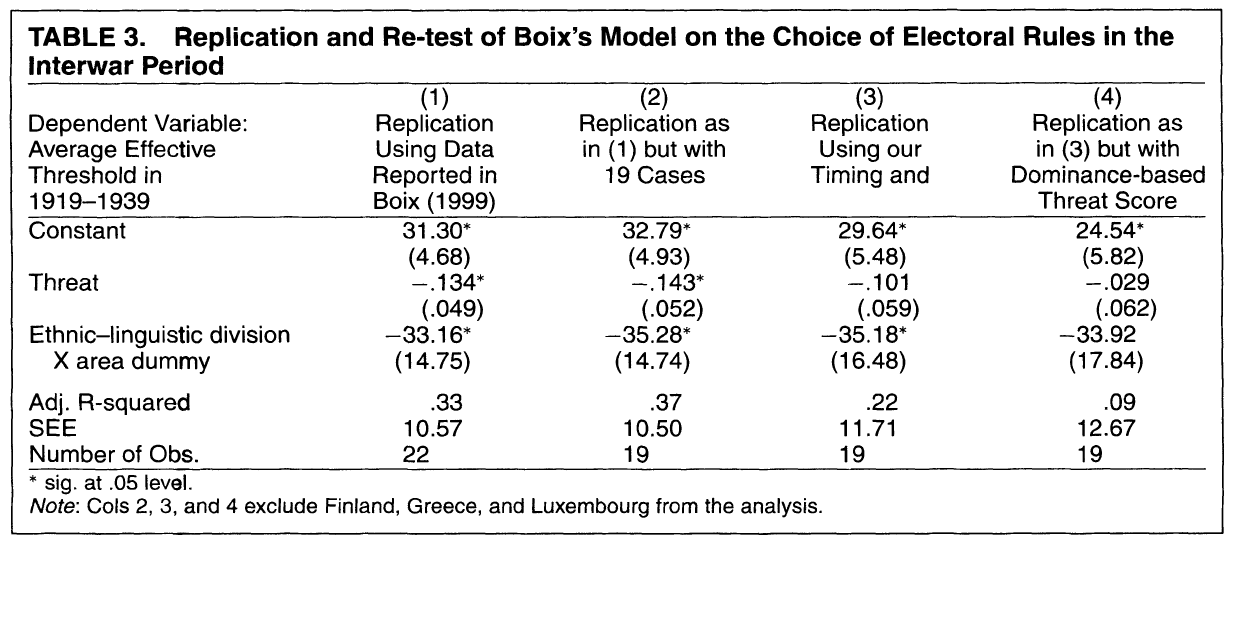
\includegraphics[width=\textwidth]{figure/CusackIversenSoskiceTable3.png}
\end{center}
}

\frame{
\frametitle{Your first analysis in R}
\noindent\texttt{
\alert<2>{library(\symbol{34}foreign\symbol{34})\\}
\alert<3>{cis <- read.dta(file.choose())[cis\$smpl==1,]\\}
\alert<4>{lm3\_1 <- lm(thresh\textasciitilde threat + fragdum,\\ data = cis)\\}
\alert<5>{lm3\_2 <- lm(thresh\textasciitilde threat + fragdum,\\ data=cis[cis\$oursmpl==1,])\\}
\alert<6>{lm3\_3 <- lm(thresh\textasciitilde threat13 + fragdum,\\ data=cis[cis\$oursmpl==1,])\\}
\alert<7>{lm3\_4 <- lm(thresh\textasciitilde stthroct2 + fragdum,\\ data=cis[cis\$oursmpl==1,])\\}
\alert<8>{lapply(ls(pattern=\symbol{34}lm\symbol{34}),\\
    function(i) round(summary(get(i))\$coef[,1:2],2))\\}
}
}

\againframe{q}

\frame<1>[label=basics]{
\frametitle{R Language Basics}
\begin{itemize}\itemsep2em
\item<1-> Everything in R is an ``object''
\item<2-> All objects have a ``class''
\item<3-> We execute functions on objects
	\begin{itemize}
	\item<3-> Functions work differently (or not at all) on different classes
	\end{itemize}
\item<4-> Functions return objects \emph{and} print to the console
\item<5-> We can then do further things with those objects
\end{itemize}
}

\frame{\frametitle{Try on your own}
Create variables:\\Do the \href{https://github.com/leeper/Rcourse/blob/gh-pages/Scripts/variables.r}{``Variables''} tutorial
}

\againframe{q}
\againframe<1-2>{basics}

\frame{\frametitle{Try on your own}
Understand R data structures:
\begin{itemize}\itemsep1em
\item \href{https://github.com/leeper/Rcourse/blob/gh-pages/Scripts/vectors.r}{``Vectors''}
\item \href{https://github.com/leeper/Rcourse/blob/gh-pages/Scripts/vectorindexing.r}{``Vector indexing''}
\item \href{https://github.com/leeper/Rcourse/blob/gh-pages/Scripts/matrices.r}{``Matrices''}
\item \href{https://github.com/leeper/Rcourse/blob/gh-pages/Scripts/lists.r}{``Lists''}
\item \href{https://github.com/leeper/Rcourse/blob/gh-pages/Scripts/dataframes.r}{``Dataframes''}
\end{itemize}
}

\againframe{q}

%\frame{\Large It's time for a five-minute break}

\againframe<2-5>{basics}

\frame{\frametitle{Try on your own}
Understand objects and printing:\\Do the \href{https://github.com/leeper/Rcourse/blob/gh-pages/Scripts/objects.r}{``Objects''} tutorial
}


\frame{
\frametitle{When things go wrong...}
\only<2->{
\begin{enumerate}\itemsep2em
\item Don't panic
\item Parsing errors versus syntax errors:
	\begin{itemize}
	\footnotesize
	\item \texttt{Error: unexpected ')' in "lm(y \textasciitilde)"}
	\item \texttt{Error in eval(expr, envir, enclos) : object 'y' not found}
	\end{itemize}
\item Google the error or warning
\item Use \href{http://stackoverflow.com/questions/tagged/r}{StackOverflow}
\end{enumerate}
}
}

\frame{
\frametitle{A script editor makes your life easier\dots}
\begin{itemize}\itemsep2em
\item Helps you understand code more easily
\item Work interactively to build a script
	\begin{itemize}
	\item R script is like a Stata do file
	\item File extension: \texttt{.R} or \texttt{.r }
	\end{itemize}
\item Write down all of your code
\item Use comments (\texttt{\#}) liberally
\end{itemize}
}


\frame{
\frametitle{\dots so let's install one}
\texttt{
\alert<2>{install.packages(\symbol{34}devtools\symbol{34})\\}
\alert<3>{library(\symbol{34}devtools\symbol{34})\\}
\alert<4>{install\_github(\symbol{34}rite\symbol{34}, \symbol{34}leeper\symbol{34})\\}
\vspace{1em}
\alert<5>{library(\symbol{34}rite\symbol{34})\\}
\alert<6>{rite()}
}
}

\againframe{q}


%\appendix

\bgroup
\setbeamercolor{background canvas}{bg=black}
\setbeamertemplate{navigation symbols}{}
\begin{frame}[plain]{}
\end{frame}
\egroup

\end{document}
